\documentclass{book}

\usepackage{listings}
\usepackage{theorem}
\usepackage{graphicx}
\usepackage{hyperref}
\usepackage{amsfonts}
\usepackage{amsmath}
\usepackage[table]{xcolor}
\usepackage{array,calc}
\usepackage{amsmath}

\newtheorem{exercise}{Exercise}


\lstset{
  language=Java,
  basicstyle=\ttfamily\footnotesize,
  numbers = left
}

\newcommand{\co}[1]{\lstinline[language=Java, basicstyle=\ttfamily]{#1}}

\begin{document}

\chapter{Digital Images}
In this course, we study techniques for analysing and processing \emph{digital images}. But how can we represent such digital images and their colors? In this chapter, we answer the aforementioned question.

\section{Image Representation}
An image can be represented as a raster or as a set of geometrical primitives.

\subsection{Raster Images}
A \emph{raster image} is a rectangular, two-dimensional grid of picture elements, more commonly known as pixels. Each pixel has a corresponding color.

Each raster image has a certain \emph{width} and \emph{height}. For example, the width of the raster image shown below is 8 and its height is 4. Therefore, the image contains 32 pixels.
\begin{center}
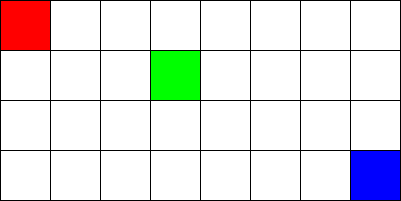
\includegraphics[scale=0.35]{rasterimage.png}
\end{center}
A common convention in raster image processing is that pixel indexing is zero-based and that the origin is located in the upper left corner. The Y-axes is therefore oriented downwards. For example, the red pixel in the image shown above is located at coordinate $(0, 0)$, the green pixel at $(3, 1)$ and the blue pixel at $(7, 3)$. $(-1, -1)$ and $(8, 8)$ are invalid coordinates for this image.

Mathematically speaking, a raster image $I$ is a two-dimensional, partial function from integer coordinates to colors:
$$I: \mathbb{N} \times \mathbb{N} \rightarrow \mathcal{C}$$
$I$ is partial as it is not defined for all pairs of natural numbers. In the remainder of this course, we will denote image functions using the letter $I$. $I(x, y)$ therefore denotes the pixel value at coordinate $(x, y)$.

Images taken by digital cameras are typically stored as raster images. For example, bitmap, png, tiff and jpeg are four popular file formats for raster images. The latter three file formats apply compression (either lossy or lossless) to reduce the file size. Png and tiff apply lossless compression meaning that the exact original image can be reconstructed from the compressed file. Jpeg supports both lossy and lossless compression.

\subsection{Vector Images}
A \emph{vector image} represents an image as a set of geometrical primitives such as polygons, lines, circles, etc. For example, consider the image shown below. 

\begin{center}

\includegraphics[scale=0.3]{smiley.png}
\end{center}

In a raster image, the color of each individual pixel would be stored. In a vector image however the smiley is represented as a large yellow circle, two small, black ovals and a black polyline (each with its own offset and transformation).

Scalable vector graphics (svg) is a xml-based file format for vector images. For example, the smiley shown above is encoded in svg as follows:  
\begin{lstlisting}[language=xml,basicstyle=\ttfamily\small]
<svg xmlns="http://www.w3.org/2000/svg" version="1.1">
  <circle cx="100" cy="100" r="100" fill="yellow"/>
  <circle cx="60" cy="35" r="15" fill="black" 
    transform="scale(1, 2)"/>
  <circle cx="140" cy="35" r="15" fill="black"
    transform="scale(1, 2)"/>
  <polyline points="60,140 70,150 130,150 140,140" 
      fill="none" stroke="black" stroke-width="3"/>
</svg>
\end{lstlisting}
Line 2 defines the circle representing the head, lines 3 to 6 the ovals representing the eyes and lines 7 and 8 the polyline representing the mouth. Scalable vector graphics are supported by most browsers (e.g. the latest versions of Firefox, Safari, Chrome, Internet Explorer and Opera).

\begin{exercise}
Save the svg file shown above as \co{smiley.svg}. Open this file in a browser. Experiment with vector images by modifying the attributes of the geometric primitives and by adding new primitives. \href{http://www.svgbasics.com}{http://www.svgbasics.com} describes how to use other geometric primitives and transformations. For example, can you replace the mouth of the smiley by a smooth line?
\end{exercise}

\begin{exercise}
Which operation do you think is easier: converting a raster to a vector image or vice versa? Why?
\end{exercise}

Most displays and printers are raster devices. Vector images must therefore be converted to raster format before being displayed. 

Vector images have a number of advantages compared to raster images. 
\begin{itemize}
  \item Each geometric shape and its corresponding configuration is stored separately. Therefore, one can  modify a single shape without affecting other shapes or loss of image quality. For example, changing the size and color of the smiley's face does not distort the eyes or mouth.
  \item One can zoom in on or enlarge a vector image without pixelation. When zooming in on a raster image, individual pixels become visible.
  \item The file size of a vector image is typically smaller than the size of a similar raster image as only shapes are stored instead of the color of each individual pixel. The difference becomes more pronounced as the width and height of the raster image increase. Small vector images however do lack the detail found in photographs.
\end{itemize}

\begin{exercise}
The portable document format (pdf) is a form of vector image. Open a pdf and zoom in on the text. Do you notice any pixelation?
\end{exercise}

%\begin{exercise}
%What is the file size of \co{smiley.svg}? Convert \co{smiley.svg} to a jpeg of size 200x200 on \href{http://www.fileformat.info/convert/image/svg2raster.htm}{http://www.fileformat.info/convert/image/svg2raster.htm}. What is the file size of this raster image? Now convert \co{smiley} to a jpeg of size 1000x1000. What is the fiel size of the produced jpeg?
%\end{exercise}

Digital cameras produce raster images. We mainly focus on analysing and processing raster images in the remainder of this course.

\section{Colors}
Each pixel in a raster image has a corresponding color. We distinguish three types of images.

\subsection{Binary Images}
A binary image contains only two colors: black and white. The color of each pixel can therefore be stored in a single bit, where 0 represents black and 1 represents white.
\begin{center}
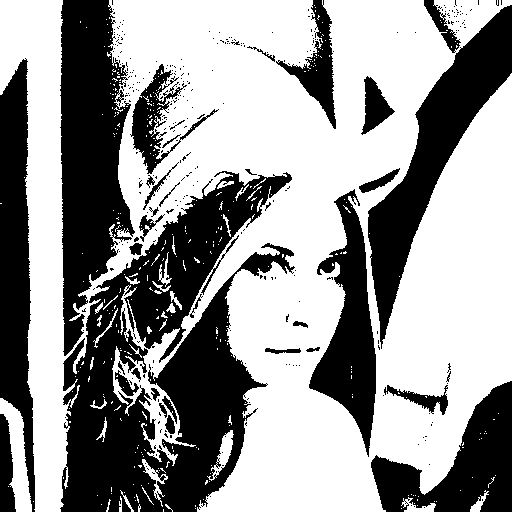
\includegraphics[scale=0.15]{lena-binary.png}
\end{center}
\begin{exercise}
How many bytes are needed to store a 100x100 binary image without compression?
\end{exercise}

\subsection{Grayscale Images}
A grayscale image only contains different shades of gray but no ``real'' colors. 
\begin{center}
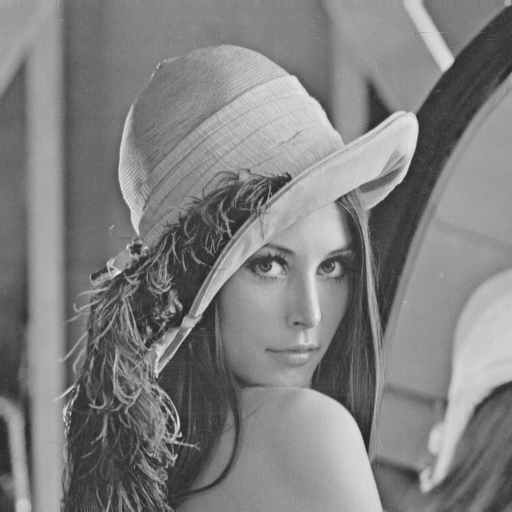
\includegraphics[scale=0.15]{lena-gray.png}
\end{center}
More specifically, the color of each pixel in a grayscale image is represented by a number between 0 and some maximum. For example, in 8-bit grayscale each pixel color is stored in 8 bits. Therefore, 8-bit grayscale can distinguish between 256 ($2^8$) different shades of gray with 255 being the maximum representing white. The $i$th column in the 8-bit grayscale image shown below displays the shade of gray represented by $i$.
\begin{center}

\includegraphics[scale=0.75]{gradient-image.png}
\end{center}
Note that binary images are grayscale images where the number of bits per pixel is one.

\begin{exercise}
How many bytes are needed to store a 100x100 8-bit grayscale image without compression?
\end{exercise}

\subsection{RGB Color Images}
Each pixel in an RGB color image has a color that is defined as a mixture of red, green and blue.
\begin{center}
\includegraphics[scale=0.15]{additive-rgb.png}
\end{center}
Red, green and blue are called the color channels or color components. Each component is encoded in a certain number of bits. For example, in 24-bit RGB color images each component is encoded into 8-bits and hence each channel can take 256 different values. The table shown below displays a number of 24-bit RGB triples together with the corresponding hexadecimal notation and color. For example, cyan is formed by combining green (255) and blue (255).

\definecolor{springgreen}{RGB}{0,255,127}
\begin{center}
\begin{tabular}{| c | c | c | c | c |}
\hline
red & green & blue & hexadecimal & color\\ \hline
0 & 0 & 0 & 0x000000 & \cellcolor{black}\\ \hline
255 & 0 & 0 & 0xFF0000 & \cellcolor{red}\\ \hline
0 & 255 & 0 & 0x00FF00 & \cellcolor{green}\\ \hline
0 & 0 & 255 & 0x0000FF & \cellcolor{blue}\\ \hline
255 & 255 & 0 & 0xFFFF00 & \cellcolor{yellow}\\ \hline
255 & 0 & 255 & 0xFF00FF & \cellcolor{magenta}\\ \hline
0 & 255 & 255 & 0x00FFFF & \cellcolor{cyan}\\ \hline
255 & 255 & 255 & 0xFFFFFF & \cellcolor{white}\\ \hline
0 & 255 & 127 & 0x00FF7F & \cellcolor{springgreen}\\ \hline
\end{tabular}
\end{center}

\begin{exercise}
How many different colors can be represented by a 24-bit RGB color pixel?
\end{exercise}

\begin{exercise}
Experiment with mixing the primary colors red, green and blue on \href{http://fys.kuleuven.be/pradem/applets/RUG/KleurenMenger/index.htm}{http://fys.kuleuven.be/pradem/applets/RUG/KleurenMenger/index.htm}. Adjust the sliders and inspect the resulting colors. What are the colors corresponding to the triples (50, 50, 50), (100, 100, 100) and (150, 150, 150)? In general, what color is formed when the red, green and blue components  are equal?
\end{exercise}

\begin{exercise}
How many bytes are needed to store a 100x100 24-bit RGB color image without compression? What is the file size in kilobyte (KB)?
\end{exercise}

\begin{exercise}
We scan a 15x10cm color photograph at 100 dots per inch (1 inch = 2.54cm). What is the file size of the resulting image (ignoring compression and metadata)? 
\end{exercise}

\subsection*{Hexadecimal}
RGB colors are often written in hexadecimal notation. Hexadecimal is a numeral system with base or radix 16. It uses 16 distinct digits: 0, 1, 2, 3, 4, 5, 6, 7, 8, 9, A, B, C, D, E, F to represent numbers. 0-9 represent the values zero to nine and A-F represent ten to fifteen. For example, the hexadecimal number 3C is equal in decimal to 60 ($=3*16 + 12$). Hexadecimal numbers are often prefixed with ``0x'' to distinguish them from decimal numbers.

A hexadecimal number can be converted to decimal by multiplying each digit with the corresponding power of 16. For example, the hexadecimal number 0xA1B2 can be written in decimal as 41394 as shown in the following derivation.
$$\begin{array}{l}
A \times 16^3 + 1 \times 16^2 + B \times 16^1 + 2 \times 16^0\\
= 10 \times 16^3 + 1 \times 16^2 + 11 \times 16^1 + 2 \times 16^0\\
= 10 \times 4096 + 1 \times 256 + 11 \times 16 + 2 \times 1\\
= 40960 + 256 + 176 + 2\\
= 41394
\end{array}$$

A decimal number can be converted to hexadecimal by repeatedly dividing by 16 until the result is 0. For example, suppose we want to convert the decimal number 1234 to hexadecimal notation. We start by dividing 1234 by 16 which yields 77 with remainder 2. This means that 2 is the least significant digit of our hexadecimal number. Dividing 77 by 16 yields 4 with remainder 13. The decimal number 13 is denoted as D in hexadecimal. This means that the second digit in our number is D. Finally, dividing 4 by 16 yields 0 with remainder 4, and hence the most significant digit is 4. Thus, the decimal number 1234 is written in hexadecimal as 0x4D2.

\begin{exercise}
Convert the following hexadecimal numbers to decimal notation: 0x5, 0x21, 0xA6, 0xFFE. Check your answers online using a hex-to-decimal converter.
\end{exercise}

\begin{exercise}
Convert the following decimal numbers to hexadecimal notation: 4, 12, 17, 200, 300. Check your answers online using an decimal-to-hex converter.
\end{exercise}

\begin{exercise}
Write a Java program to convert decimal numbers to hexadecimal and vice versa.
\end{exercise}

Each hexadecimal digit represents four binary digits. For example, 0x7 can be written in binary as 0111, 0xA as 1010, 0xE as 1110. Hence, the primary use of hexadecimal notation is as a human-friendly representation of binary-coded values. In particular, each byte can be represented by two hexadecimal digits. For example, the binary number 11111111 (using 8 bits so exactly one byte) can be written in hexadecimal as 0xFF and in decimal as 255.

\begin{exercise}
In the Java programming language, \co{int}  is a primitive data type. Each \co{int} is stored into 32 bits. How many hexadecimal digits are needed to describe the bits of an integer?
\end{exercise}

In 24-bit RGB images, each pixel is stored in 24 bits with 8 bits per channel. These 24 bits are often written in hexadecimal notation. For example, the bits that represent the color magenta can be written in hexadecimal as 0xFF00FF. 

\subsection{Other color representations}
In this course, we will mostly use the 24-bit RGB color representation. However, there exist other color representations. For example, HSV is a color representation where each color consists of a hue, a saturation and a value. An advantage of HSV compared to RGB is that it is easier to modify the brightness of a pixel without affecting its hue.

CMYK is a subtractive color model, used in color printing, where the primary colors cyan, magenta, yellow and black are combined to from colors.
\begin{center}
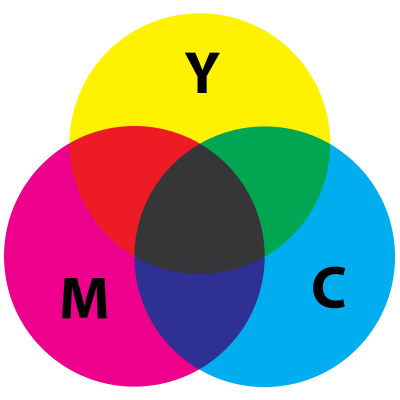
\includegraphics[scale=0.15]{cmyk.png}
\end{center}

\end{document}